Обратим внимание сразу, что данные преобразования можно применять к любым функциям. Также мы можем применять сразу несколько преобразований, получая более сложные функции.

\subsection{Преобразование $y = f (x + c)$, c   – число}

Примеры: $y=\sqrt{x+3}$, $y=\frac{1}{x+3}$

\begin{itemize}
    \item В случае $c > 0$ график функции $y = f (x)$ переносится влево на расстояние $|c|$
    \item В случае $c < 0$ график функции $y = f (x)$ переносится вправо на расстояние $|c|$
\end{itemize}

\begin{figure}[h!]
	\begin{minipage}[h]{0.49\linewidth}
		\center{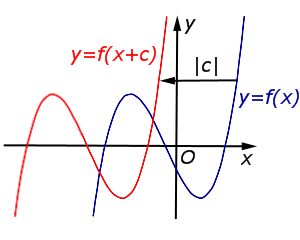
\includegraphics[width=0.7\linewidth]{img/pr1.png} \\ $c > 0$ сдвиг по оси OX влево}
	\end{minipage}
	\hfill
	\begin{minipage}[h]{0.49\linewidth}
		\center{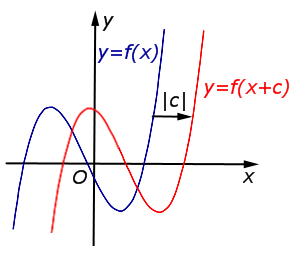
\includegraphics[width=0.7\linewidth]{img/pr2.png} \\ $c < 0$ сдвиг по оси OX вправо}
	\end{minipage}
	\label{ris:image1}
\end{figure}

\subsection{Преобразование $y = f (x) + c$, c   – число}

Примеры: $y=\sqrt{x}+3$, $y=\frac{1}{x}+3$

\begin{itemize}
    \item В случае $c > 0$ график функции $y = f (x)$ переносится вверх на расстояние $|c|$
    \item В случае $c < 0$ график функции $y = f (x)$ переносится вниз на расстояние $|c|$
\end{itemize}

\begin{figure}[h!]
	\begin{minipage}[h]{0.49\linewidth}
		\center{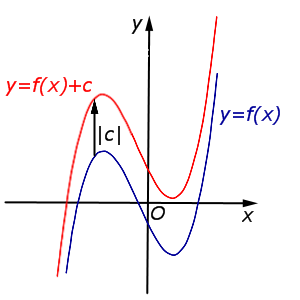
\includegraphics[width=0.7\linewidth]{img/pr3.png} \\ $c > 0$ сдвиг по оси OY вверх}
	\end{minipage}
	\hfill
	\begin{minipage}[h]{0.49\linewidth}
		\center{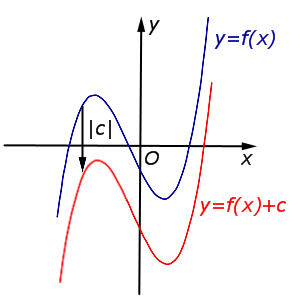
\includegraphics[width=0.7\linewidth]{img/pr4.png} \\ $c < 0$ сдвиг по оси OY вниз}
	\end{minipage}
	\label{ris:image1}
\end{figure}

\subsection{Преобразование отражения  $y = - f(x)$ и $y = f (-x)$}

Примеры: $y=-\sqrt{x}$, $y=\sqrt{-x}$

\begin{itemize}
    \item $y = - f(x)$ \\
    График функции $y = f (x)$ симметрично отражается относительно оси OX.
    \item $y = f (-x)$ \\
    График функции   $y = f (x)$ симметрично отражается относительно оси OY.
\end{itemize}

\begin{figure}[h!]
	\begin{minipage}[h]{0.49\linewidth}
		\center{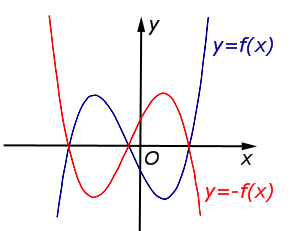
\includegraphics[width=0.7\linewidth]{img/pr5.png} \\ $y = - f(x)$ отражение от OX}
	\end{minipage}
	\hfill
	\begin{minipage}[h]{0.49\linewidth}
		\center{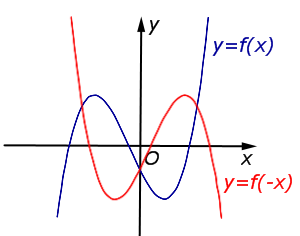
\includegraphics[width=0.7\linewidth]{img/pr6.png} \\ $y = f (-x)$ отражение от OY}
	\end{minipage}
	\label{ris:image1}
\end{figure}

\subsection{Преобразование $y = f (kx)$, k   – число}

Пример: $y=\sqrt{3x}$, $y=\frac{1}{3x}$

\begin{itemize}
    \item В случае $k > 1$ происходит сжатие графика функции $ y = f (x)$ в k раз к оси OY.
    \item В случае   $0 < k < 1$   происходит растяжение графика функции $y = f (x)  $ в  $\frac{1}{|k|}$ раз от оси OY.
\end{itemize}

\begin{figure}[h!]
	\begin{minipage}[h]{0.49\linewidth}
		\center{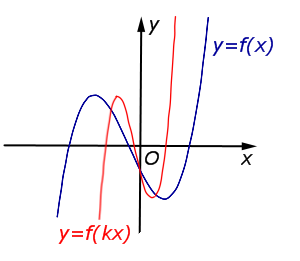
\includegraphics[width=0.7\linewidth]{img/pr7.png} \\ $k > 1$ - сжатие по OX (к OY)}
	\end{minipage}
	\hfill
	\begin{minipage}[h]{0.49\linewidth}
		\center{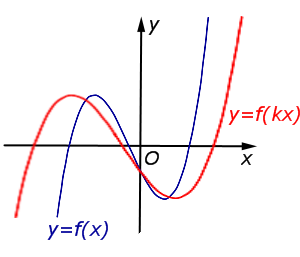
\includegraphics[width=0.7\linewidth]{img/pr8.png} \\ $0 < k < 1$ растяжение по OX (от OY)}
	\end{minipage}
	\label{ris:image1}
\end{figure}

(?) Что будет с графиком при $k<0$? при $-1<k<0$?

\subsection{Преобразование $y = k f (x)$, k   – число}

Пример: $y=3\sqrt{x}$, $y=\frac{3}{x}$

\begin{itemize}
    \item В случае   $k > 1$   происходит растяжение графика функции
    $y = f (x)$ в k раз от оси Ox.
    \item В случае   $0 < k < 1$   происходит сжатие графика функции
    $y = f (x)$ в $\frac{1}{|k|}$ раз к оси Ox.
\end{itemize}

\newpage

\begin{figure}[h!]
	\begin{minipage}[h]{0.49\linewidth}
		\center{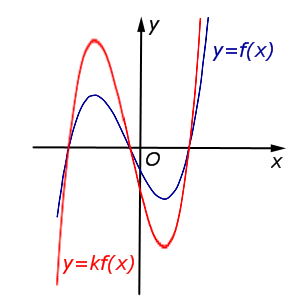
\includegraphics[width=0.7\linewidth]{img/pr11.png} \\ $k > 1$ - растяжение по OY (от OX)}
	\end{minipage}
	\hfill
	\begin{minipage}[h]{0.49\linewidth}
		\center{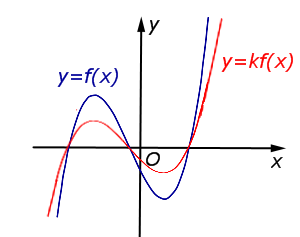
\includegraphics[width=0.9\linewidth]{img/pr12.png} \\ $0 < k < 1$ сжатие по OY (к OX)}
	\end{minipage}
	\label{ris:image1}
\end{figure}

\subsection{Преобразование модуля $y = | f (x)|$ и $y = f (| x|)$}

\begin{itemize}
    \item $y = | f (x)|$. Часть графика функции $y = f (x)$, расположенная в области $y>0$, остаётся на месте. Часть графика функции   y = f (x), расположенная в области $y < 0$, симметрично отражается относительно оси Ox.
    \item $y = f (| x|)$. Ось Oy является осью симметрии
    графика функции   $y = f (| x|)$. Часть графика функции   y = f (x), расположенная в области $x>0$ остаётся на месте. Часть графика функции $y = f (| x|)$, расположенная в области $x < 0$,
    получается из части графика, расположенной в области $x>0$ при помощи симметричного отражения относительно оси Oy.
\end{itemize}

\begin{figure}[h!]
	\begin{minipage}[h]{0.49\linewidth}
		\center{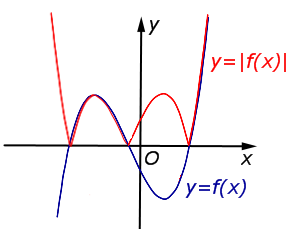
\includegraphics[width=0.7\linewidth]{img/pr15.png} \\ $y = | f (x)|$- отражение от ОХ}
	\end{minipage}
	\hfill
	\begin{minipage}[h]{0.49\linewidth}
		\center{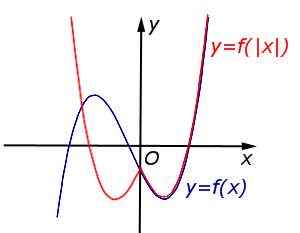
\includegraphics[width=0.7\linewidth]{img/pr16.png} \\ $y = f (| x|)$ отражение от OY}
	\end{minipage}
	\label{ris:image1}
\end{figure}

Пример:
\begin{figure}[h!]
	\begin{minipage}[h]{0.49\linewidth}
		\center{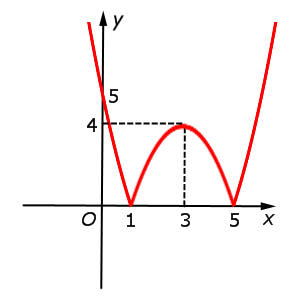
\includegraphics[width=0.6\linewidth]{img/pr_ex1.png} \\ $y = | x^2 - 6x + 5|$}
	\end{minipage}
	\hfill
	\begin{minipage}[h]{0.49\linewidth}
		\center{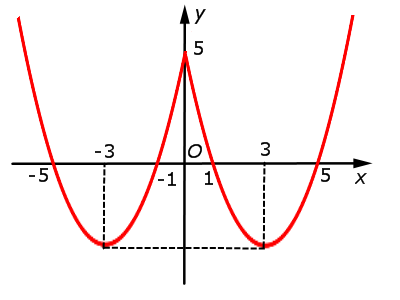
\includegraphics[width=0.65\linewidth]{img/pr_ex2.png} \\ $y = x^2 - 6 |x| + 5$}
	\end{minipage}
	\label{ris:image1}
\end{figure}
